%----------------------------------------------------------------------------
% Start
%----------------------------------------------------------------------------

\documentclass{article}

\usepackage{graphicx} % Required for the inclusion of images 
\usepackage{tocloft}
\usepackage[nottoc,numbib]{tocbibind} % Reference in TOC and numbered 
\usepackage{url} % References include URLs
\usepackage{mathtools} % Math stuff
\usepackage[export]{adjustbox}
\usepackage{hyperref} % Makes links actually work!
\usepackage[toc,numberedsection]{glossaries}
\usepackage{geometry}

\renewcommand{\cftsecleader}{\cftdotfill{\cftdotsep}} 
\renewcommand{\labelenumi}{\alph{enumi}.}

\geometry {a4paper, left = 30mm}
\renewcommand{\baselinestretch}{1.5}
\setlength{\parskip}{1em}
\setlength\parindent{0pt} % Removes all indentation from paragraphs


%----------------------------------------------------------------------------
% Document Information
%----------------------------------------------------------------------------

\begin{document}

\title{Giguesaur: Game Logic}
\author{Ashley Manson}
\date{\today}

\begin{titlepage}
\clearpage
\maketitle
\thispagestyle{empty} % Remove page number from title page

\begin{center}
\large 
Co-Workers: Joshua La Pine \& Shahne Rodgers\\
Supervisors: Geoff Wyvill \& David Eyers\\

\vspace*{1\baselineskip} % Skip a line

Department of Computer Science\\
University of Otago

\end{center}

\end{titlepage}

\pagenumbering{roman}
%----------------------------------------------------------------------------
% Abstract
%----------------------------------------------------------------------------

\begin{abstract}
Giguesaur is a collaborative, augmented-reality jigsaw puzzle game which is
played on iPads. This report will go into detail of the many aspects of the game
logic behind the Giguesaur application, how the game is rendered to the screen,
how a player would interact with the virtual jigsaw puzzle, and how Joshua,
Shahne and I completed the project.
\end{abstract}

%----------------------------------------------------------------------------
% Define Glossary
%----------------------------------------------------------------------------
\newglossaryentry{OpenGL} { name={OpenGL}, description={is a graphics
    application programming interface used to render 2D and 3D graphics} }

\newglossaryentry{OpenGLES} { name={OpenGL ES}, description={is for Embedded
    Systems graphics programming, used a lot on mobile devices, and is a subset
    of OpenGL} }

\newglossaryentry{iOS} { name={iOS}, description={is a mobile operating system
    created and developed by Apple} }

\newglossaryentry{Android} { name={Android}, description={is a mobile operating
    system based on the Linux kernel that is developed by Google} }

\newglossaryentry{Xcode} { name={Xcode}, description={is an integrated
    development environment built by Apple and is used to develop Mac and iOS
    applications} }

\newglossaryentry{GameBoard} { name={Game Board}, description={is a marker
    tracker in the real world that the puzzle pieces are superimposed upon and
    where the player interacts with the puzzle pieces} }

\newglossaryentry{Mac} { name={Macintosh}, description={is the name of computers
    created and developed by Apple, shortened to Mac. They run on OS X, Apples
    computer operating system} }

\newglossaryentry{OpenCV} { name={OpenCV}, description={is a computer vison
    library aimed at real-time computer vison} }

\newglossaryentry{Neighbour} { name={Neighbour}, description={is a piece that
    shares an edge to another piece} }

\makeglossaries

%----------------------------------------------------------------------------
% Table of Contents
%----------------------------------------------------------------------------

\clearpage
\tableofcontents
\clearpage

\pagenumbering{arabic}
\setcounter{page}{1}

%----------------------------------------------------------------------------
% Introduction
%----------------------------------------------------------------------------

\section{Introduction}

Our vision for our completed Giguesaur application was allowing a classroom of
children, each with their own iPad, to run around and solve a virtual jigsaw
puzzle together. Imagine a classroom full of kids where they are all trying to
work on a single conventional jigsaw puzzle; such a scheme is in no way
practical. Giguesaur allows you to view a virtual jigsaw puzzle in the real
world through the iPad's screen and camera. The main goal of our project was to
make an application that is fun for children to play.

% Overview of the project
\subsection{Overview}
The Giguesaur project is an application that is run on iPads that is rendered
using augmented reality, I will talk more of this in section
\ref{ssec:AugReality}. This allows a group of people to collaboratively solve a
virtual jigsaw puzzle. The puzzle is assembled on a \gls{GameBoard} in the real
world, where it is a checkerboard marker for the iPad's camera to track. The
jigsaw puzzle pieces that are rendered on screen will be shown to be
superimposed upon the game board. The user is able to interact with the jigsaw
puzzle by tapping the iPads screen, rotating and moving the iPad around while
looking at the marker. The touch gestures and movement with the iPad allows the
user to pick up, place and move the jigsaw puzzle pieces in the game. The iPad's
are connected to a central server ran on a \gls{Mac} (Mac), which allows for
multiple people to interact with the jigsaw puzzle.

% Format of the project
\subsection{Project Format}
Due to the complexity and size of the Giguesaur project, it had to be divided
into three different components, as no single person would have been able to
achieve the aims and goals of the project in a single year. Joshua La Pine was
in charge of developing the computer vison component of the project, which
allows for the puzzle pieces to be rendered on top of the game board in the real
world. Shahne Rodgers took charge of the networking component of the project,
which allows more than one player to interact with the jigsaw puzzle. Finally my
part of the project was to develop the game logic and render the game to the
iPad's screen.

% Background including what a puzzle is and other games
\subsection{Background}
There are many existing jigsaw puzzle games such as Magic Jigsaw Puzzles
\cite{ref:MagicJigsaw} and Jigsaw Puzzle \cite{ref:JigsawPuzzle}. The existing
games are limited in the way they look because they use an orthographic
projection to render the jigsaw puzzles on a two dimensional board on the
computer screen. The puzzle pieces of the jigsaw puzzle are flat on the
screen. The player can only look at the virtual puzzle from top down, there is
no depth. This is a factor that does not work for the Giguesaur project, we want
it to appear that the virtual pieces exist in the real world. Another limitation
of the existing games is how the puzzles are solved, the pieces have to be
assembled into a grid. Farms And Animals Puzzles \cite{ref:FarmPuzzle} have the
grid layout shown in Figure \ref{fig:FarmsAnimals}, all the pieces have an
absolute location to be placed in. For Giguesaur I have made it possible for the
jigsaw puzzle to be solved anywhere on the game board, be it in the centre or
off in a corner.

\begin{figure}[ht]
\begin{center}
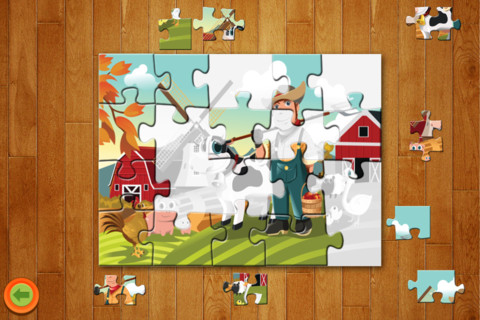
\includegraphics[width=0.75\textwidth]{images/FarmAnimalsJigsawImage}
\caption{Screenshot of Farms And Animals Puzzles \cite{img:FarmPuzzle}.}
\label{fig:FarmsAnimals}
\end{center}
\end{figure}

% iOS compared to Android
\subsection{Why iOS?}
\gls{iOS} is an operating system made for Apple's mobile devices, which all
present a similar interface for the user. \gls{Android} is an open source
operating system based on Linux. It runs in many version on many different
devices \cite{ref:AndroidDevices}. The devices that Android runs cover a wide
range of screen resolutions and processing power \cite{ref:AndroidHardware}. We
had decided that the Giguesaur game would be developed for iOS for several
reasons. iOS hardware was more standardized than Android, as Apple are the only
developers of iPhones and iPads \cite{ref:iOSHardware}. It made it easy for us
to write the code. We knew that we would be relatively sure that what we
developed would work on the majority of iOS devices, at least the ones with
cameras. We could not be certain that any Android development of an application
would work. It would have not been possible, in a fourth year project, to ensure
that the application would work on all kinds of Android devices. Apple also have
a powerful and intuitive integrated development environment (IDE) called
\gls{Xcode}. With its detailed profiling tools and other features such as
interface builders, it made it easier for us to develop and quickly prototype
our ideas for the application.

% Brief explaination of AR and examples
\subsection{Augmented Reality} \label{ssec:AugReality}
Augmented reality is the idea of superimposing virtual objects on top of the
real world that looks convincing enough for someone to believe what they are
seeing is actually physically real. Figure \ref{fig:ARDefender} has a game being
played on a simple coffee table while looking through an iPhone. The game is a
simple tower defence game where the user aims where the tower shoots by moving
the iPhone around the table while the camera has a marker on the table in
view. The marker on the table, of which is hidden under the projection of the
defence tower, is what allows the game to obtain the required information to
correctly pose the game objects onto the table. The idea of augmented reality is
what we based the Giguesaur game on, using marker trackers to correctly pose the
puzzle pieces onto the game board so it gives the idea that we are interacting
with jigsaw puzzle pieces in the real world.

\begin{figure}[ht]
\begin{center}
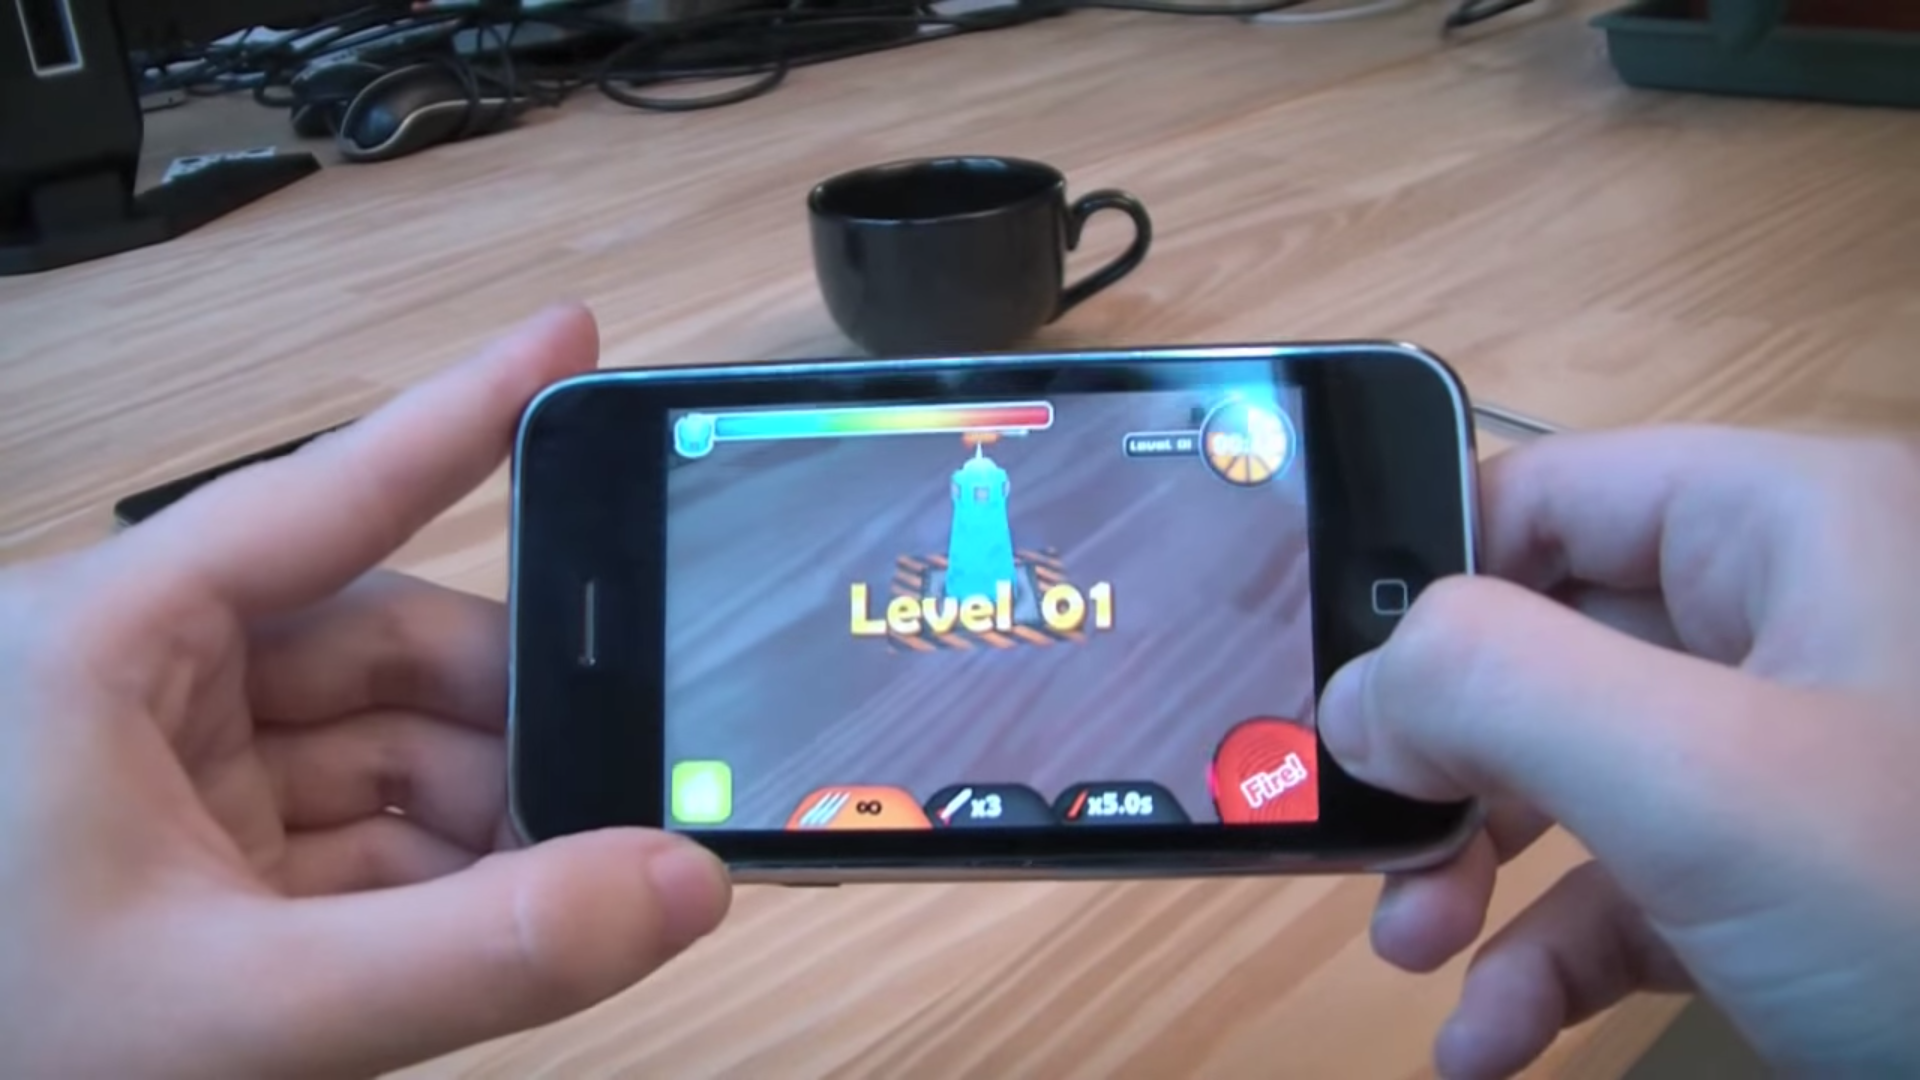
\includegraphics[width=0.75\textwidth]{images/ARDefenderImage}
\caption{Screenshot of ARDefender \cite{img:ARDefender}.}
\label{fig:ARDefender}
\end{center}
\end{figure}

% Brief introduction on my work
\subsection{Game Logic}
I was in charge of developing the game logic for the Giguesaur game. This meant
I had to create the logic for how jigsaw puzzle pieces interacted with each
other and how the user interacted with the game. The jigsaw puzzle is made up of
a grid with a specific number of rows and columns, where each part of the grid
is a piece. Each piece has four edges, and an edge either has a neighbouring
piece or not. If a piece edge has a \gls{Neighbour}, it is given the ID of its
neighbour for that edge, if it has no neighbour, than the value -1 is given to
that edge. An edge of a piece can be open, meaning it has not joined to its
neighbour or closed meaning it has joined to its neighbour, or if the edge has
no neighbour it is unjoinable, meaning it can't join or be joined to another
piece for that edge. An unjoinable edge is the outside edge of the puzzle. Each
piece of the puzzle has a unique ID, a position in space, or an x, y coordinate
on the board, and a rotation with a value between 0 and 360 degrees. The z
coordinate is assumed to be 0, so it is ignored. This is what makes up the game
logic for the jigsaw puzzle. I made up my own data structure to store these
details. All the pieces that are in the game are stored in an array, where the
piece ID is the index of the array the piece is stored. The x, y coordinate
determines where on the board the piece is displayed and the rotation affects
the orientation of the piece. The board that the pieces are placed on has a
width and length, which are along the x, y axis, which confines where the puzzle
pieces can be placed, as all the pieces have an x, y coordinate. Figure
\ref{fig:GameLogic} presents a diagram of the game logic in the game.

\begin{figure}[ht]
\begin{center}
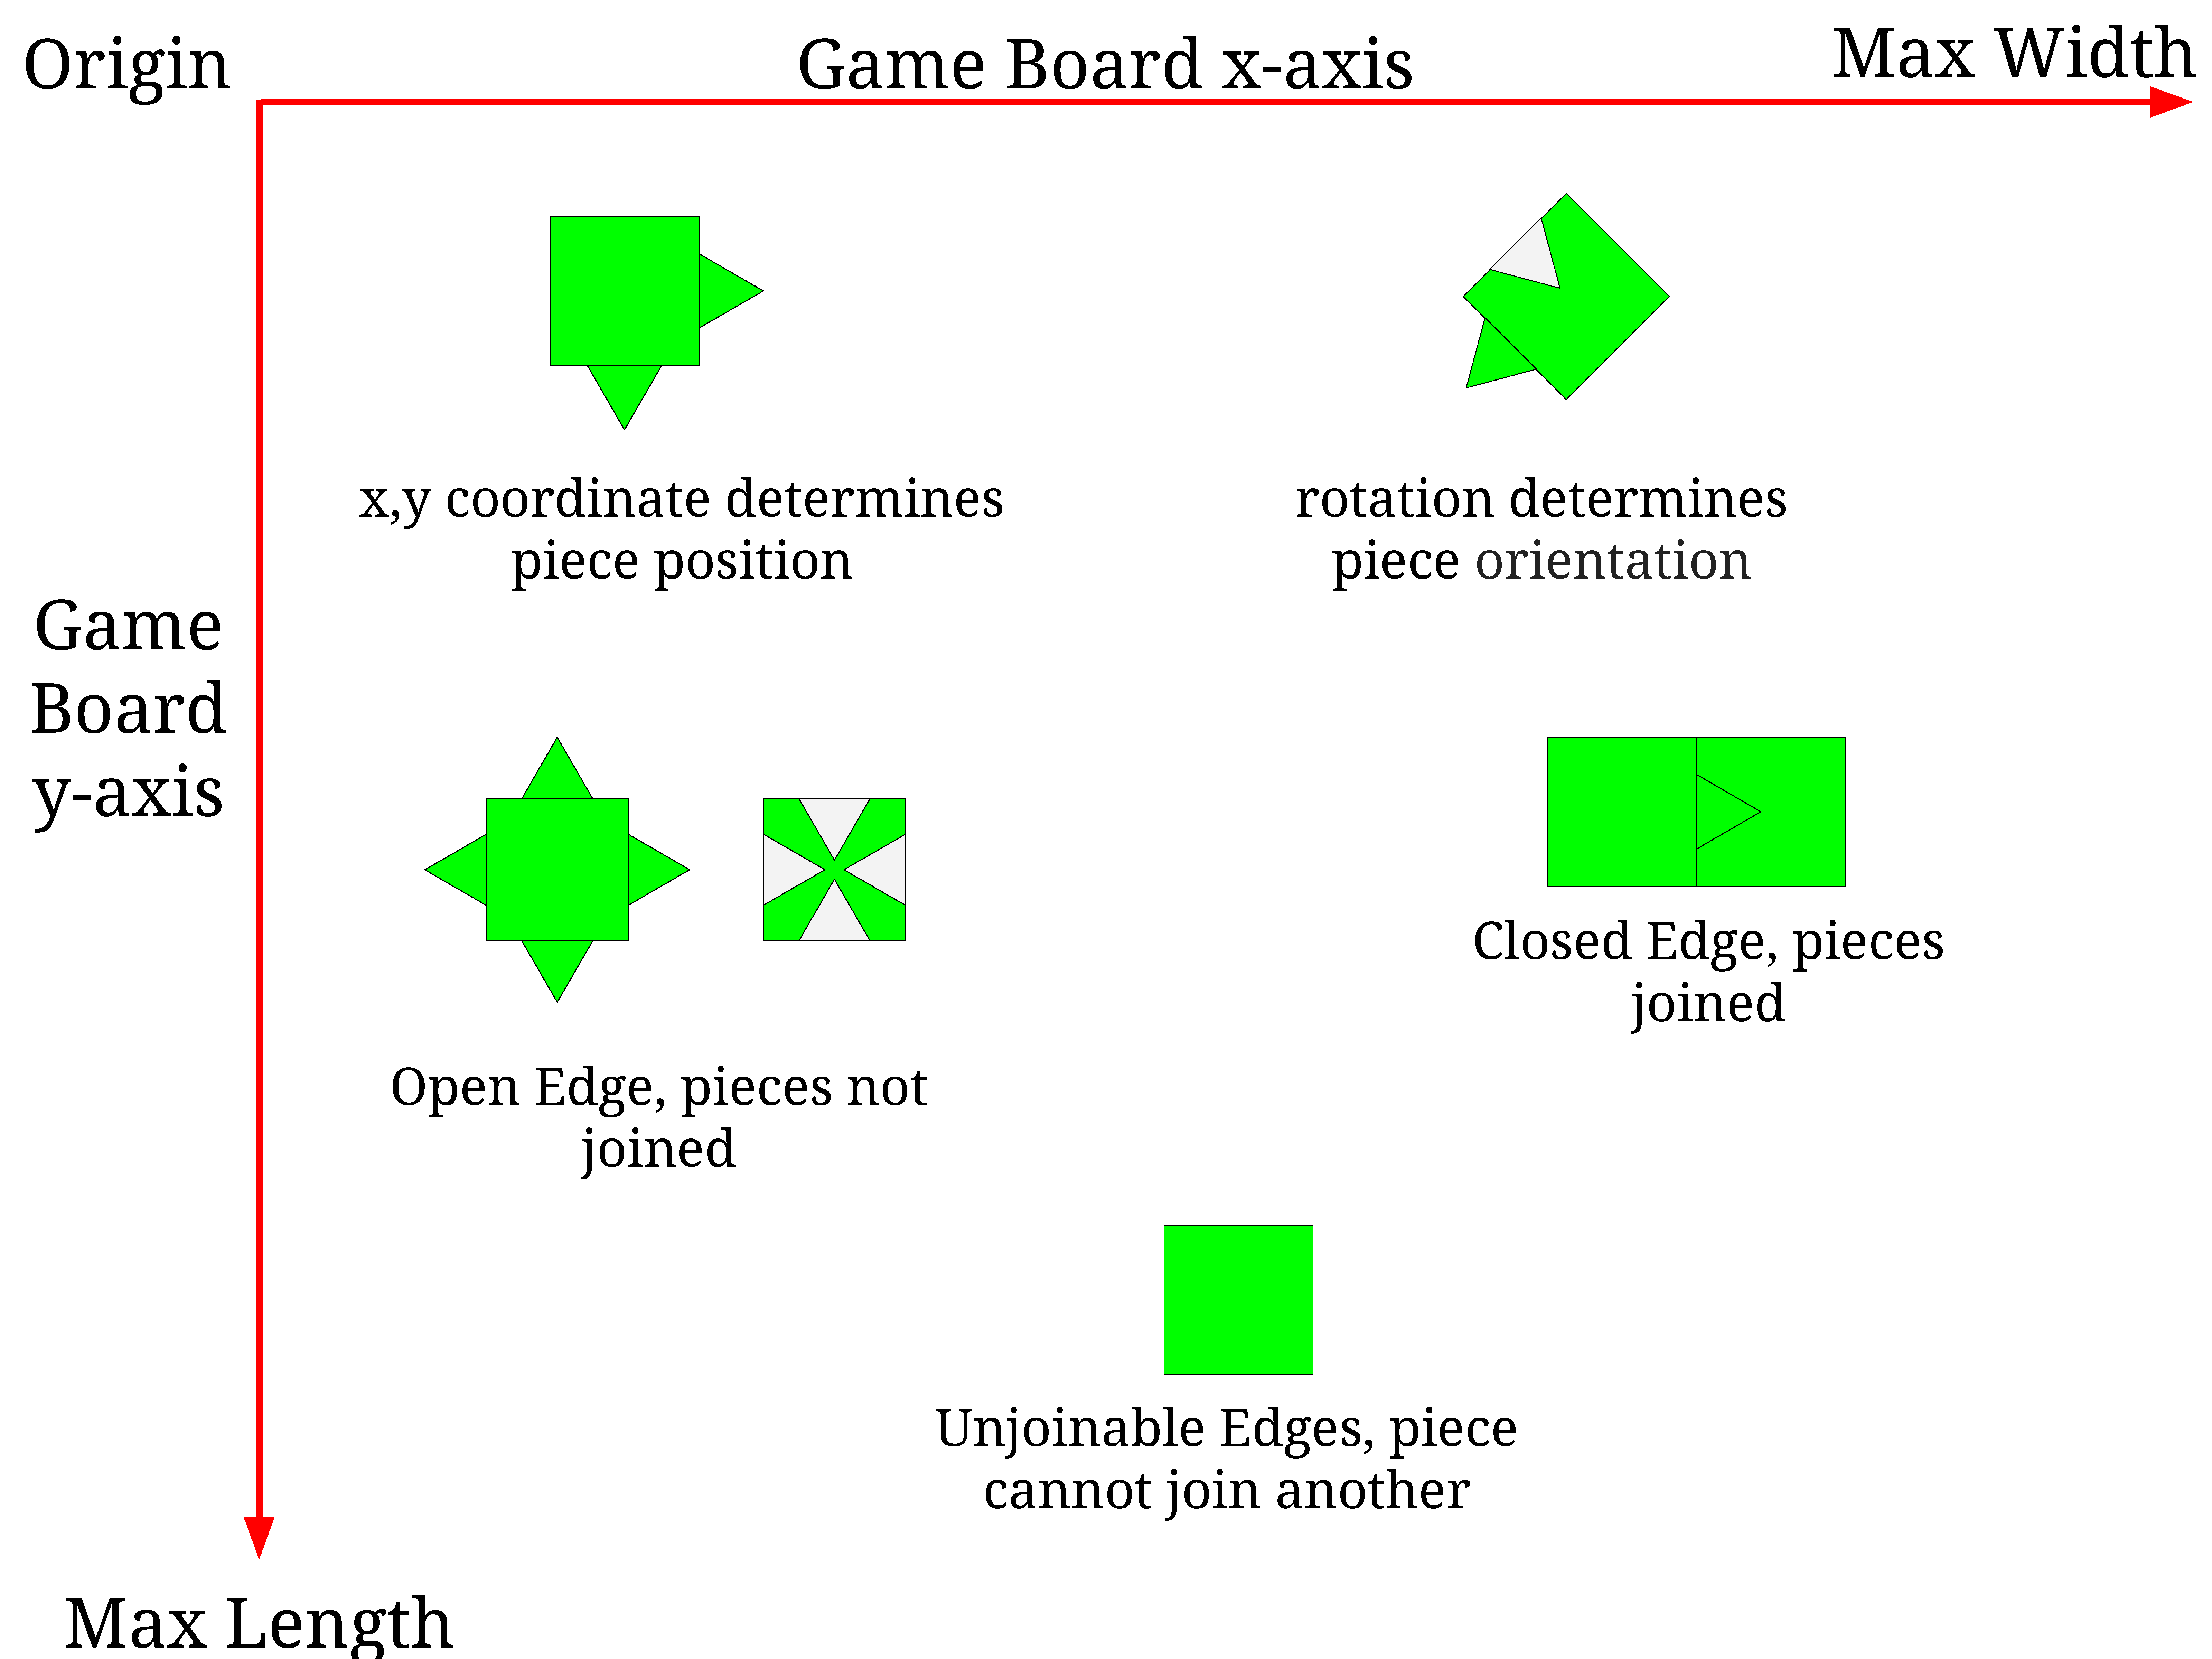
\includegraphics[width=0.85\textwidth, center]{images/GameLogicDiagram}
\caption{Diagram of the Game Logic.}
\label{fig:GameLogic}
\end{center}
\end{figure}

%---------------------------------------------------------------------------
% Achievements
%---------------------------------------------------------------------------

\section{Achievements}

% Work done on Mac
\subsection{Prototype}
In the beginning of the project I developed a prototype of the Giguesaur game
for MacOS, using some simple \gls{OpenGL} routines to render the game. Working on the
MacOS version helped when I was creating the game logic for the application, as
I could quickly test my ideas for the game logic such as jigsaw puzzle piece
interaction. It also allowed me to quickly try out ideas that would be time
consuming on an iOS. What I achieved with the prototype is the following; It
allowed me to get to grips with OpenGL, such as calling all the drawing routines
and getting to grips with the coordinate system, I completed and implemented all
the game mechanics for the game, such as picking up and dropping pieces and the
snapping of pieces, and I also tested out using a perspective projection to
render the game in a proper perspective. Figure \ref{fig:MacBuild} shows what
the game looks like with a perspective projection. The broken up picture of the
puppy \cite{img:OpenGLPuppy} represents the jigsaw puzzle pieces, the green
background represents the game board the pieces are places on, and the white
boarders on the edge of the game board is the `out of bounds' area of the game
board, where the pieces could not be placed. It demonstrates pieces being
snapped together, as some of the jigsaw pieces are directly adjacent.

\begin{figure}[ht]
\begin{center}
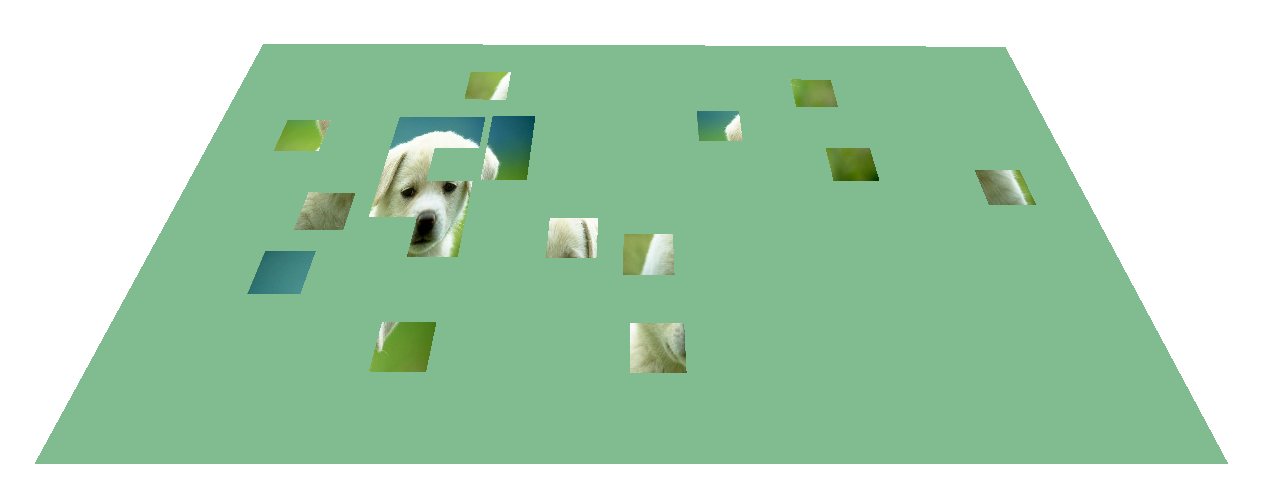
\includegraphics[width=1.2\textwidth,center]{images/MacBuildImage}
\caption{Screenshot of a prototype running on the Mac.}
\label{fig:MacBuild}
\end{center}
\end{figure}

% What the game can do
\subsection{Game Mechanics}

% The logic for piece snapping
\subsubsection{Snapping Pieces}
I wanted to enable a feature that allowed pieces to snap together. Meaning if a
piece was in a specified distance from its neighbour it would snap to it. The
piece being placed back on the board would move so that the two pieces were
right next to each other, which is shown in the Java Jigsaw Puzzle game made by
Centurio \cite{ref:SourceJigsaw}. This also has the added bonus of not having to
rely on the user to carefully place pieces together. The way the check is made
to see if two pieces should snap together is by comparing the distances between
the corresponding corner points, and if the distances are less than the snap
variable, the pieces snap together. If the piece being put back on the board is
being snapped to its left neighbour piece, the original piece top left point and
the neighbour's top right point are checked, as well as the original piece
bottom left point and the neighbour's bottom right point. The reason two
distances are checked is to make sure that piece rotations are taken into
consideration when snapping pieces together, so as to avoid an unusual snap
where a piece rotated 90 degrees snaps to its neighbour not rotated. When a
piece is snapped to another piece, the piece saves the rotation of its neighbour
as its own, so that when the change is rendered, they both have the same
rotation when beside each other. Figure \ref{fig:PieceSnapping} shows the piece
snapping mechanic with a diagram. For a puzzle to be considered solved, all the
pieces should be snapped to their corresponding neighbours. Once a piece has
snapped to its neighbour, a variable for that edge is set as closed, as well as
the neighbour's edge. So if a piece has snapped to its right neighbour, its
right edge is set as closed and the neighbour's left edge is set as closed. The
check to see if the puzzle has been solved goes through all the pieces' edges to
see if they are all closed.

\begin{figure}[ht]
\begin{center}
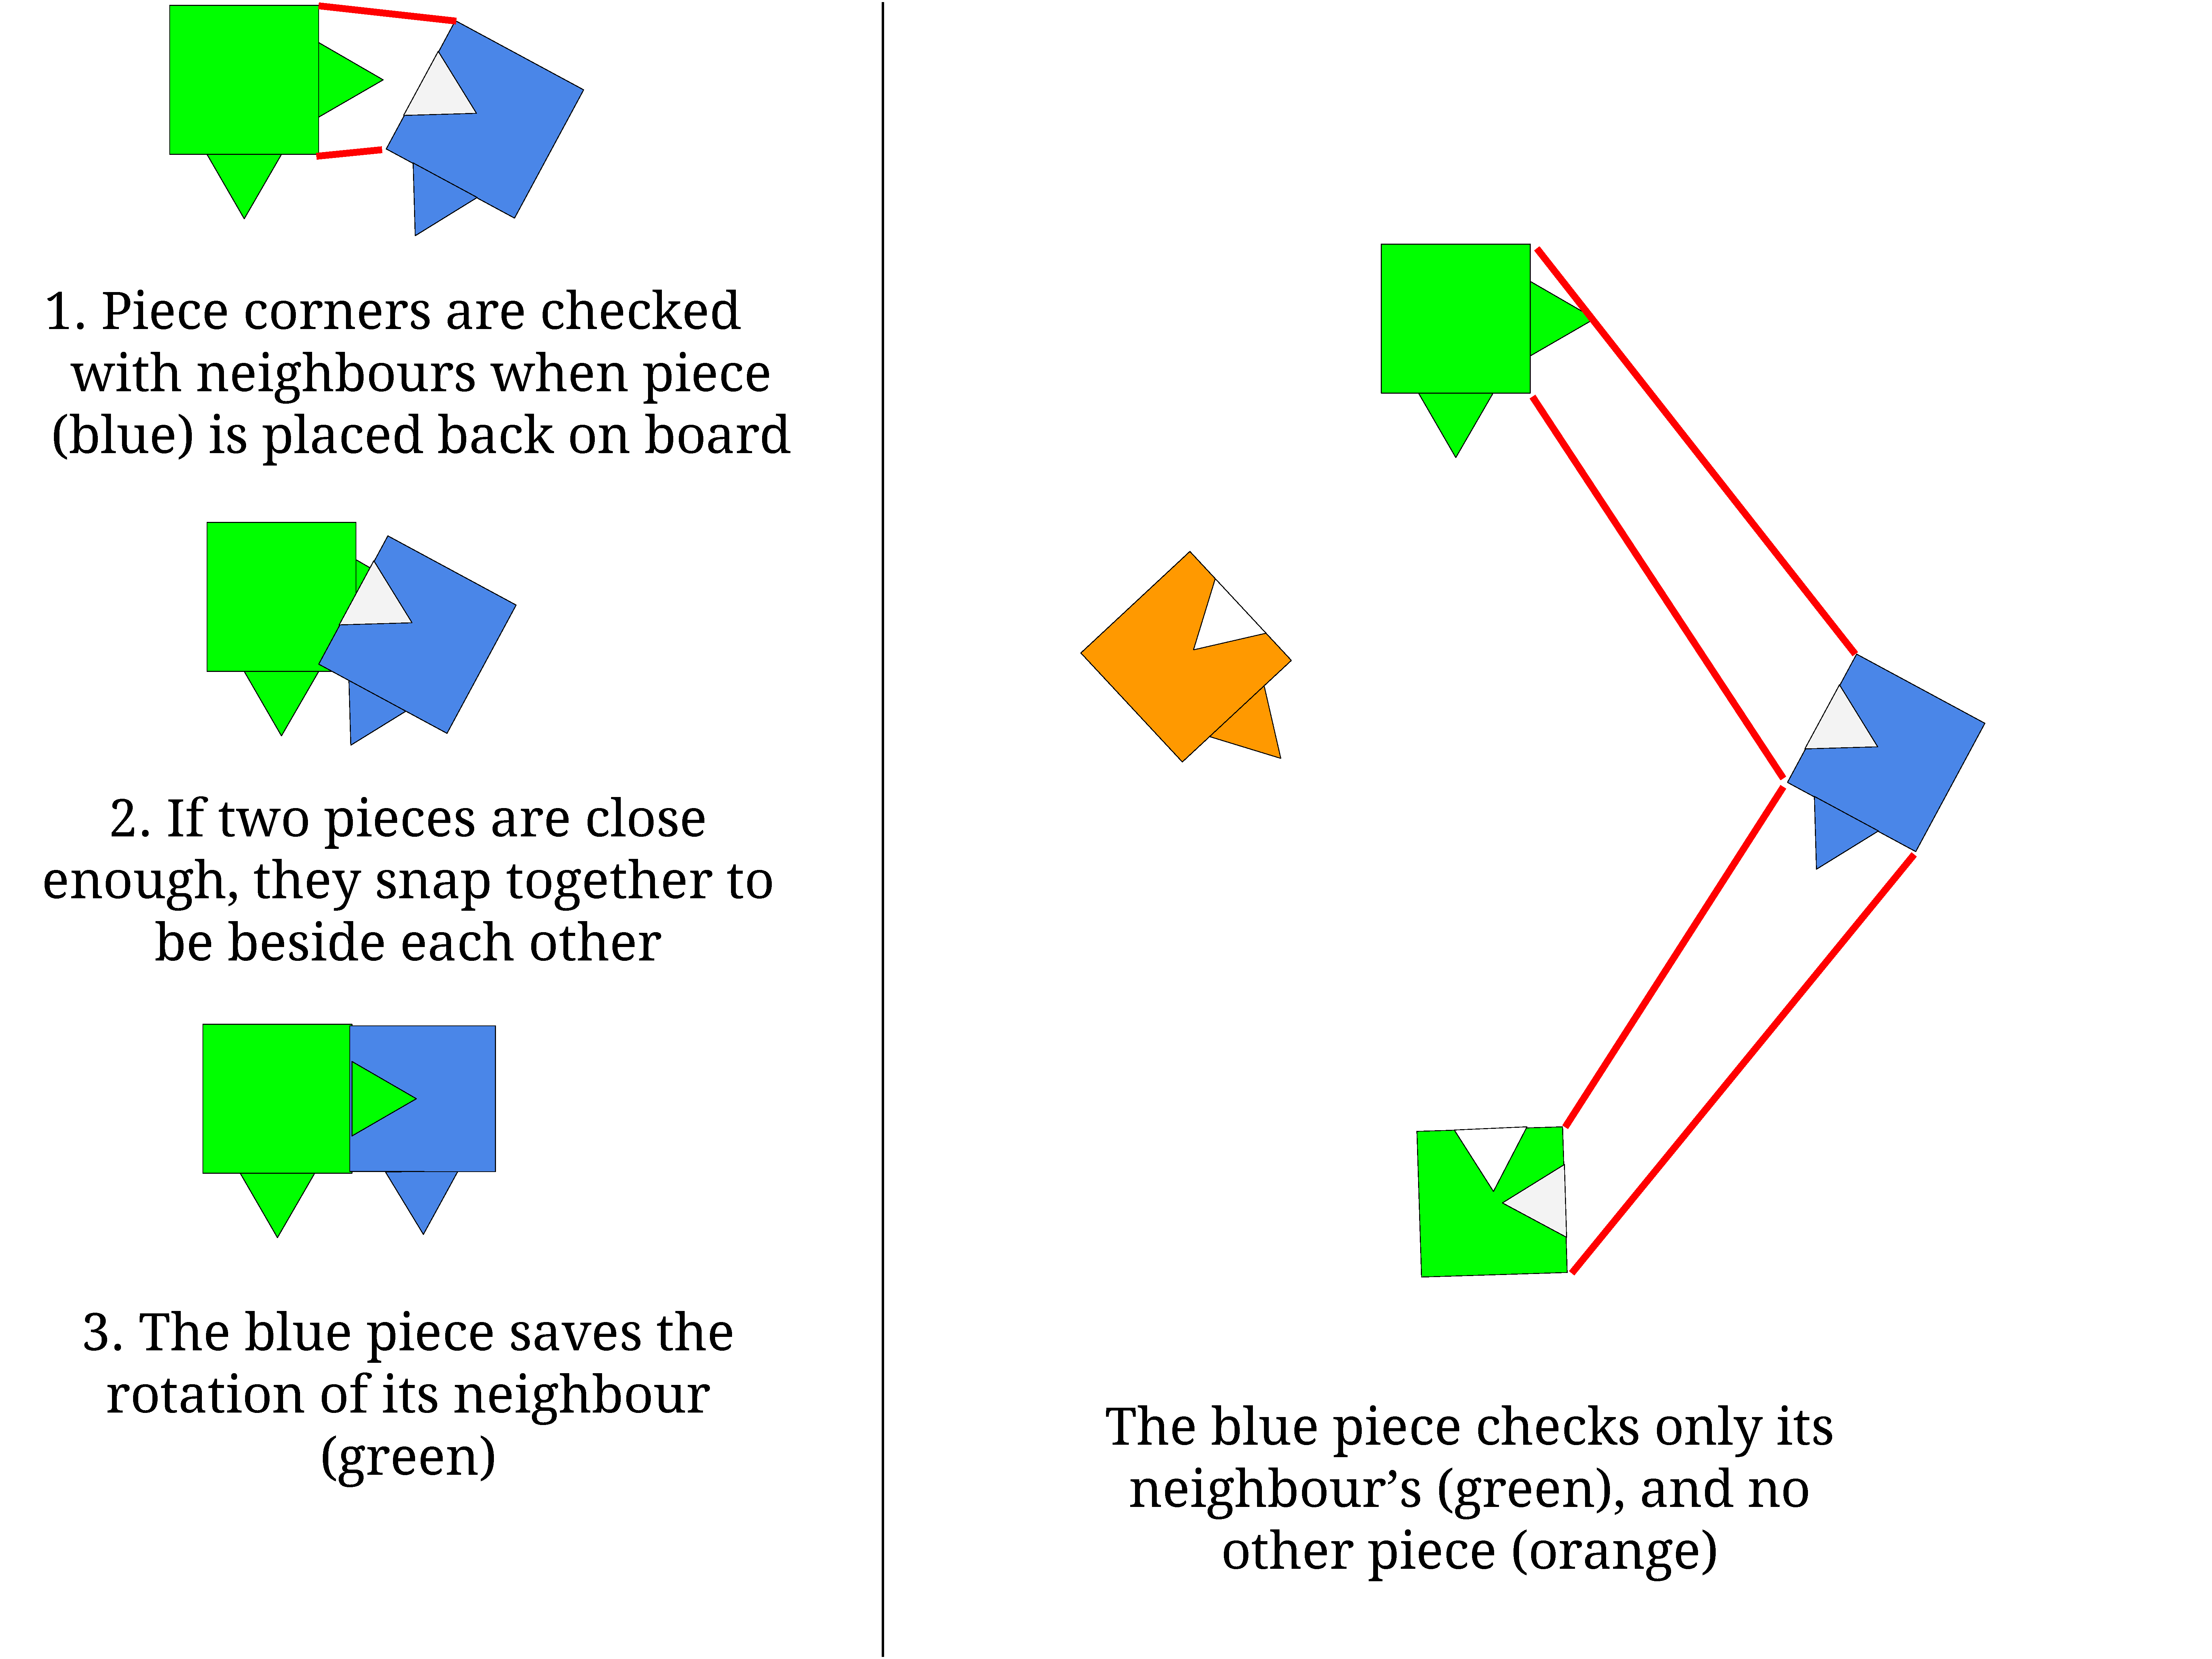
\includegraphics[width=0.85\textwidth, center]{images/PieceSnappingDiagram}
\caption{Diagram of the Piece Snapping.}
\label{fig:PieceSnapping}
\end{center}
\end{figure}

% How piece rotations are handled
\subsubsection{Piece Rotations}
Each piece has an x, y coordinate which defines where on the game board the
pieces is rendered, they also have a rotation variable that defines how the
piece is oriented on the game board. The rotation is around the z axis, where
the z axis is pointing out from the screen. The addition of rotation for puzzle
pieces added some complications to the logic of the game, in particular how I
calculated the distance between pieces for snapping as well as rendering the
pieces on screen with the correct rotations. Originally when I calculated the
distance between pieces I had been doing a simple check to see if the pieces
corner coordinates plus the length of a piece was in the range of the corner
coordinates of its neighbour. This failed to work when piece rotations were
added, as adding the side length to the coordinates did not take into
consideration the rotation. As a replacement, I now calculate the distance
between piece corners using Euclidean distance formula: 

\begin{equation*}
\begin{aligned}
d = \sqrt{(x_o - x_n)^2 + (y_o - y_n)^2}
\end{aligned}
\end{equation*}

Where $d$ is the distance, $x_o$ and $y_o$ are the coordinates of the original
piece, and $x_n$ and $y_n$ are the piece's neighbour coordinates. As I take two
distance measurements for each corner coordinates, the rotation of the pieces no
longer affect the calculation of the distances.\\

To apply the rotation to the piece itself I use the following simple formula:

\begin{equation*}
\begin{aligned}
x' = \cos(\theta) \times (x - x\_cen) - \sin(\theta) \times (y - y\_cen) + x\_cen\\ 
y' = \sin(\theta) \times (x - x\_cen) + \cos(\theta) \times (y - y\_cen) + y\_cen
\end{aligned}
\end{equation*}

Where $x$ and $y$ are the piece corner coordinates, $x\_cen$ and $y\_cen$ are
the piece centre coordinates, $\theta$ is the piece rotation in radians, and
$x'$ and $y'$ are the new corner coordinates. I applied this formula for all four
corners of a piece to get the correct rotated piece coordinates.

% The Logic for picking up and dropping pieces
\subsubsection{Picking Up and Placing Pieces}
To pick up a piece the user taps the image of a piece on the screen. That piece
is then stored in the user's `inventory' and they are no longer able to pick up
another piece, until they have placed the piece that they are holding back onto
the board. The inventory is a term I am using to state if the user is holding or
not holding a piece, as it is possible to easily check if it is empty or
not. The screen x, y coordinate from a finger tap is converted to a board x, y
coordinate, z is ignored as it is assumed to be 0. If this is close enough to a
piece then that piece is added to the user's inventory. When the user is holding
a piece, it is moved to the iPads centre of the screen and projected onto the
board. This means the user has to rotate and move the iPad around to move the
piece around the board. Once the user taps the screen again, where the piece is
projected on the board, is where the piece will be placed.

% Porting to iPad including changes and problems incountered
\subsection{Port to iPad}
Once I had established a working prototype for the Mac, the next step was to
port the code to an iPad. The port proved to be more difficult than I had
initially predicted. Firstly, OpenGL is handled completely differently with iOS
than on a Mac, as it requires the use of \gls{OpenGLES}, of which I had no
experience with before. OpenGL ES is a subset of OpenGL, which applies a number
of different methods to do rendering in comparison. When using OpenGL ES with
iOS, there is a lot of set up code that is required for any rendering to take
place. Set up like getting a reference to OpenGL ES context was required. As I
had to learn the fundmentals of OpenGL ES, I based a lot of my set up code from
Wenderlich tutorial \cite{ref:RayOpenGL} on how to create an OpenGL ES 2.0
application for iOS. Secondly, the majority of the libraries I had written for
the Mac prototype had to be re-worked and re-written to work with iOS, as some
issues like data structures were not compatible across the different
environments. For example an `NSPoint' on Mac cannot be used on iOS, instead it
is replaced with `CGPoint'. The initial port to iOS did not have a perspective
projection, which is shown in figure \ref{fig:iPadPort}. This was serious
progress to get the application onto an iPad.

\begin{figure}[ht]
\begin{center}
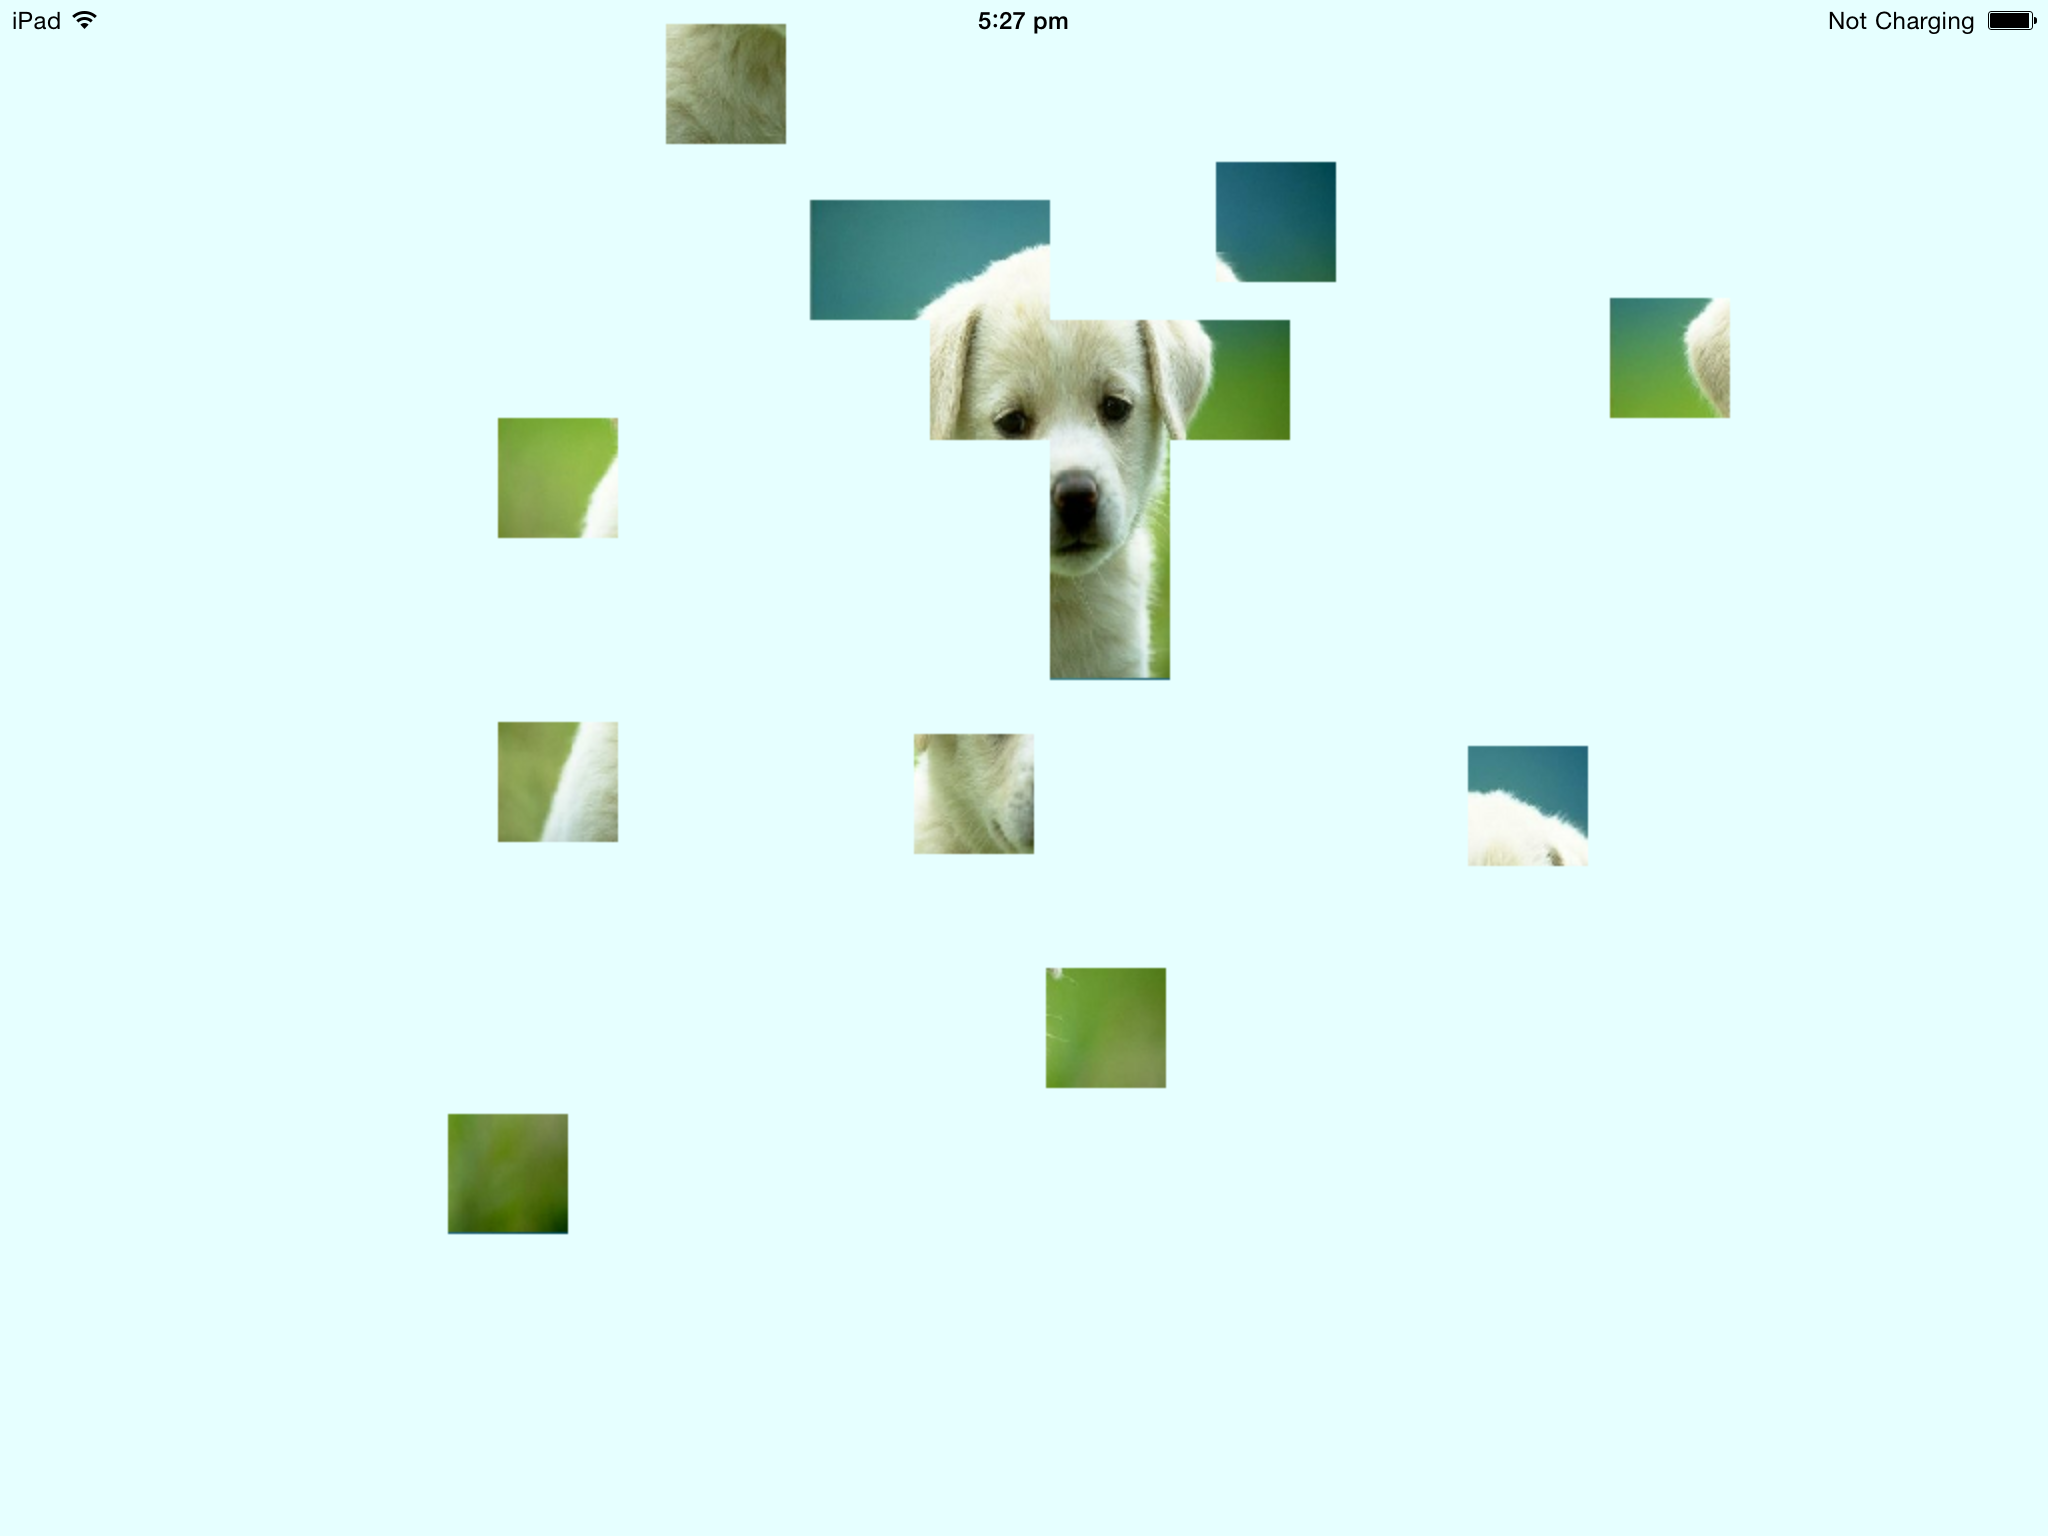
\includegraphics[width=0.95\textwidth]{images/iPadPortImage}
\caption{Screenshot of the first port to iOS.}
\label{fig:iPadPort}
\end{center}
\end{figure}

% Integrating with others including problems incountered
\subsection{Integration}
After Shahne, Josh, and I had spent the first semester working on our individual
components of the Giguesaur project, it was decided it was time to begin the
integration of the three components. It was predicted this would be a difficult
process and would take a lot of time to get everything working together. As per
the prediction, integration did take a lot of time. Not only did we have issues
of some of our code not being compatible, either by inconsistent data types or
incorrect implementations of routines, but other issues popped up such as OpenGL
and \gls{OpenCV} having issues working together. There was little to no issue with
Shahne's and my part of the integration process. On the other hand, Josh and I
were having consistent trouble getting our parts working together. It resulted
in Josh and my code being closely integrated, as we had to work together to get
the application to properly render to the iPads' screen. The following
subsections will go into more detail for my part being integrated with the two
team members.

\subsubsection{Network and Game Logic}
For the game logic to work with the networking component, the game logic that
handled piece snapping and checking for the puzzle being solved had to be moved
into the server code. The reason for this is that all players in a game had to
be getting the same information of piece locations as everyone else. As the
piece snapping code has the chance to change the coordinates of pieces it had to
be placed in the server. When a piece did snap, all clients connected to the
server got the updated piece location, so that it could be reflected when the
game rendered the pieces in their correct places. The code that checks when a
puzzle is solved seemed logical to put it with the server code. When it finds
that the puzzle has been solved, the server can alert all players of this
situation.\\

When a player attempts to pick up/place a piece on the game board, the client
has to ask the server if this is a legal action or not. This was a simple change
with my code to make this work. The logic for picking up and placing pieces will
call the routines from the networking component of the code. Once the server
responds, than my code will either pick up/place the piece or take no action
based on the responce. Shahne had already prepared for this change to the code,
so this was smooth integration of our parts of the project.\\

The only issue that occurred when integrating the network and game logic was
that I had stored all my piece locations as floats, while Shahne had stored the
pieces coordinates as integers. This meant that when the clients asked the
server if it was legal to place a piece in a certain place, the server would
store the locations as integers, and update all clients of a possibly incorrect
location. This seems quite innocent at first as the lost information is quite
small. However my code that calculated piece snapping has a fractional component
as a result after it computes. An integer would lose this information, which
shows if pieces were rotated to an obscure angle, the result would calculate a
float, the server however would interpret these as integers. The pieces than
could have the possibility to snap together incorrectly and be offset from each
other showing a visible line between them. The fix was to refactor the integer
locations into floats.

\subsubsection{Vision and Game Logic}
The integration of the vision and game logic did not go as smoothly as we would
have liked. The challenge here was to have the puzzle pieces rendered on top of
the game board in the real world. We had Josh's OpenCV code computing a
model-view matrix which was passed to my OpenGL code. The model-view matrix
would be used to correctly transform and change the perspective of the rendering
routines to have the pieces rendered upon the game board. This failed however,
as when we put this plan into pratice the puzzle pieces dissappeared from
view. Development on the project came to a halt as we tried to fix the issue,
but after a lot of time was spent attemping to solve the problem, we decided to
have OpenCV render the puzzle pieces instead, so we could move on with the rest
of the project.\\

\iffalse
The first issue we encountered when integrating the vision and game logic
components was trying to get the puzzle pieces rendered over top of the video feed
coming from the camera. The issue we found here was that OpenCV was showing the
video feed on a preview layer, which was seperate from the layer that OpenGL was
rendering to. So when we attempted to get the layers to work together, either
the OpenCV layer would cover the OpenGL layer, or vice versa, meaning one layer
was always hidden from view. Something we tried was to have the OpenGL layer use
a transparent background, with the hopes that we would be able to see the video
feed behind the OpenGL layer. However, what was behind the transparent
background was just a white background which was the OpenGL default layer
colour.\\

Due to the fact it didn't seem possible to have the use of two layers
simultaneously we decided to have OpenCV create an image for each video frame,
and with each frame, send it to the OpenGL rendering code to use as the
background image for the OpenGL layer and load it in as a texture. Another issue
arose from this change, for some reason that I was unable to fix, the image
being sent from OpenCV was overriding the already-loaded image for the
puzzle. So when the application first started, the picture of the puppy would
show up correctly, but as soon as the OpenCV routines kicked into gear and
started sending images to OpenGL, the image of the puppy seemed to disappear and
the base colour of the puzzle pieces was the only thing being rendered of the
puzzle. So we fixed one issue of not seeing what the camera could see but
introduced another problem.\\

As I could not figure out why one texture was being overridden by the other, I
decided to put trying to fix this issue on hold and move along with trying to
get the pieces showing in perspective and superimposed over the game board, as
the pieces were still showing up but with no texture on them. The issue that
arose from here was the computation of the model-view matrix. What we tried to
do was have OpenCV compute the matrix so that we could use it display the puzzle
pieces in perspective. However due to either a fault in Josh's code, or mine,
the calculated model-view matrix failed to set the pieces in a perspective
projection, nor would the pieces show up on screen at all. It seemed that what
ever we did to try and integrate the OpenGL with OpenCV would be met with
failure.\\

Due to our problems of trying to get the vision and game rendering working
together, it was decided that OpenCV would be used to render the puzzle pieces
being superimposed on the game board. For this to work, the vision code gets a
reference to the pieces array, gets and calculates the correct coordinates for
the pieces in world space, than using some simple OpenCV drawing routines, draws
the pieces on top of the game board. This allowed for not only rendering the
pieces in a correct perspective, but also solving the issue of the puzzle
textures not appearing, meaning pieces were rendering correctly. However due to
OpenGL and OpenCV having different coordinate systems, the textures of the
puzzle pieces were appearing flipped when they were rendered to the screen.
Lucklily though this was an easy fix which just required reversing the texture
coordinates of the pieces so that they appeared correctly.\\
\fi

The different coordinate systems of OpenGL and OpenCV resulted in reverse logic
for snapping of puzzle pieces. As I had written my routines with the y-axis
going bottom-up as OpenGL does it, OpenCV has the y-axis going top-down. The
change to my code that I had to do to make this work was when calculating
whether a piece can snap to its up/down neighbour, reverse the result, so when a
piece would have snapped above a piece, it will now snap below it.\\

Now the rendering and setting up of the frames is being handled by the OpenCV
routines, and my OpenGL code is being used to render the frames to the iPad's
screen after each frame update. 

% Rendering of the game
\subsection{Rendering}
I used OpenGL to apply the rendering of the Mac prototype build and the initial
port to iOS, however in the final integrated application OpenCV was being used
to create an image that is passed to the OpenGL code for it to be rendered to
the screen. The reason it is done this way is because the puzzle piece textures
have to be copied on top of the frame coming in from the camera, which requires
some extra processing to ensure the textures are shown correctly, rather than
having the puzzle pieces being rendered over the video feed coming from the
camera. Once the client receives an image file from the server, the OpenCV
routines take the file and convert it into a OpenCV image matrix for
processing. As the main image makes up the entire puzzle texture, it has to be
split up into sections for each puzzle piece that needs to be displayed on the
game board. The number of pieces determine the number of sections there will be
as each puzzle piece will need its own section of the texture. Then for each
puzzle piece, if it is meant to be displayed currently, the OpenCV routines will
copy the associated section of the texture to the image frame.

%---------------------------------------------------------------------------
% Results
%---------------------------------------------------------------------------

\section{Results}
We have managed to build a working application. The following video shows a
small demonstration of the Giguesaur application:
\url{https://www.dropbox.com/s/ronq5lmhca4h04c/Giguesaur.mp4?dl=0}. The video is
hosted on Dropbox. Figure \ref{fig:iPadFinal} is two screenshots from different
perspectives from two iPads. Both iPads are able to see the same puzzle being
rendered upon the game board. You are able to pickup and place down puzzle
pieces. The puzzle can be solved by having all the pieces join up to their
corresponding neighbours. The code for the complete project is available at:
\url{https://github.com/ShahneRodgers/Giguesaur/releases/tag/v1.0}.

\begin{figure}[ht]
\begin{center}
\centerline{
\includegraphics[width=0.5\textwidth]{images/iPadFinalImage1}
\includegraphics[width=0.5\textwidth]{images/iPadFinalImage2}
}
\caption{Screenshot of the final build running on two different iPads.}
\label{fig:iPadFinal}
\end{center}
\end{figure}

%---------------------------------------------------------------------------
% Conclusion
%---------------------------------------------------------------------------

\section{Conclusion}

% Final Wrap Up
\subsection{Discussion}
The Giguesaur application is working, though there are still couple problems
with the finished product. The performance of the application is slow, as it
runs at a low five frames a second. This is not ideal as this causes issue when
interacting with the puzzle on screen. If you were to move the iPad away from
the marker it tracks, it would grind to a halt and stall. It often takes too
long to recover for it to be reasonable, so it does not make for a fun game. Due
to the low frame rate, it can be difficult to pickup and place puzzle pieces. A
group of players are able to play with the same jigsaw puzzle, though we have
only tested this with two iPads as that's all we have. One player is able to
pickup a piece and the other player would be able to see that piece disappear
from the game board. The two players are able to work together to solve the
virtual jigsaw puzzle. Using the iPad's camera, they are able to see the puzzle
pieces on top of the real world game board. Though we were met with challenges
and problems, I believe we have achieved what was set out from the original aims
and objectives; to build an augmented reality jigsaw puzzle game where a number
of people can play together. 

\begin{figure}[ht]
\begin{center}
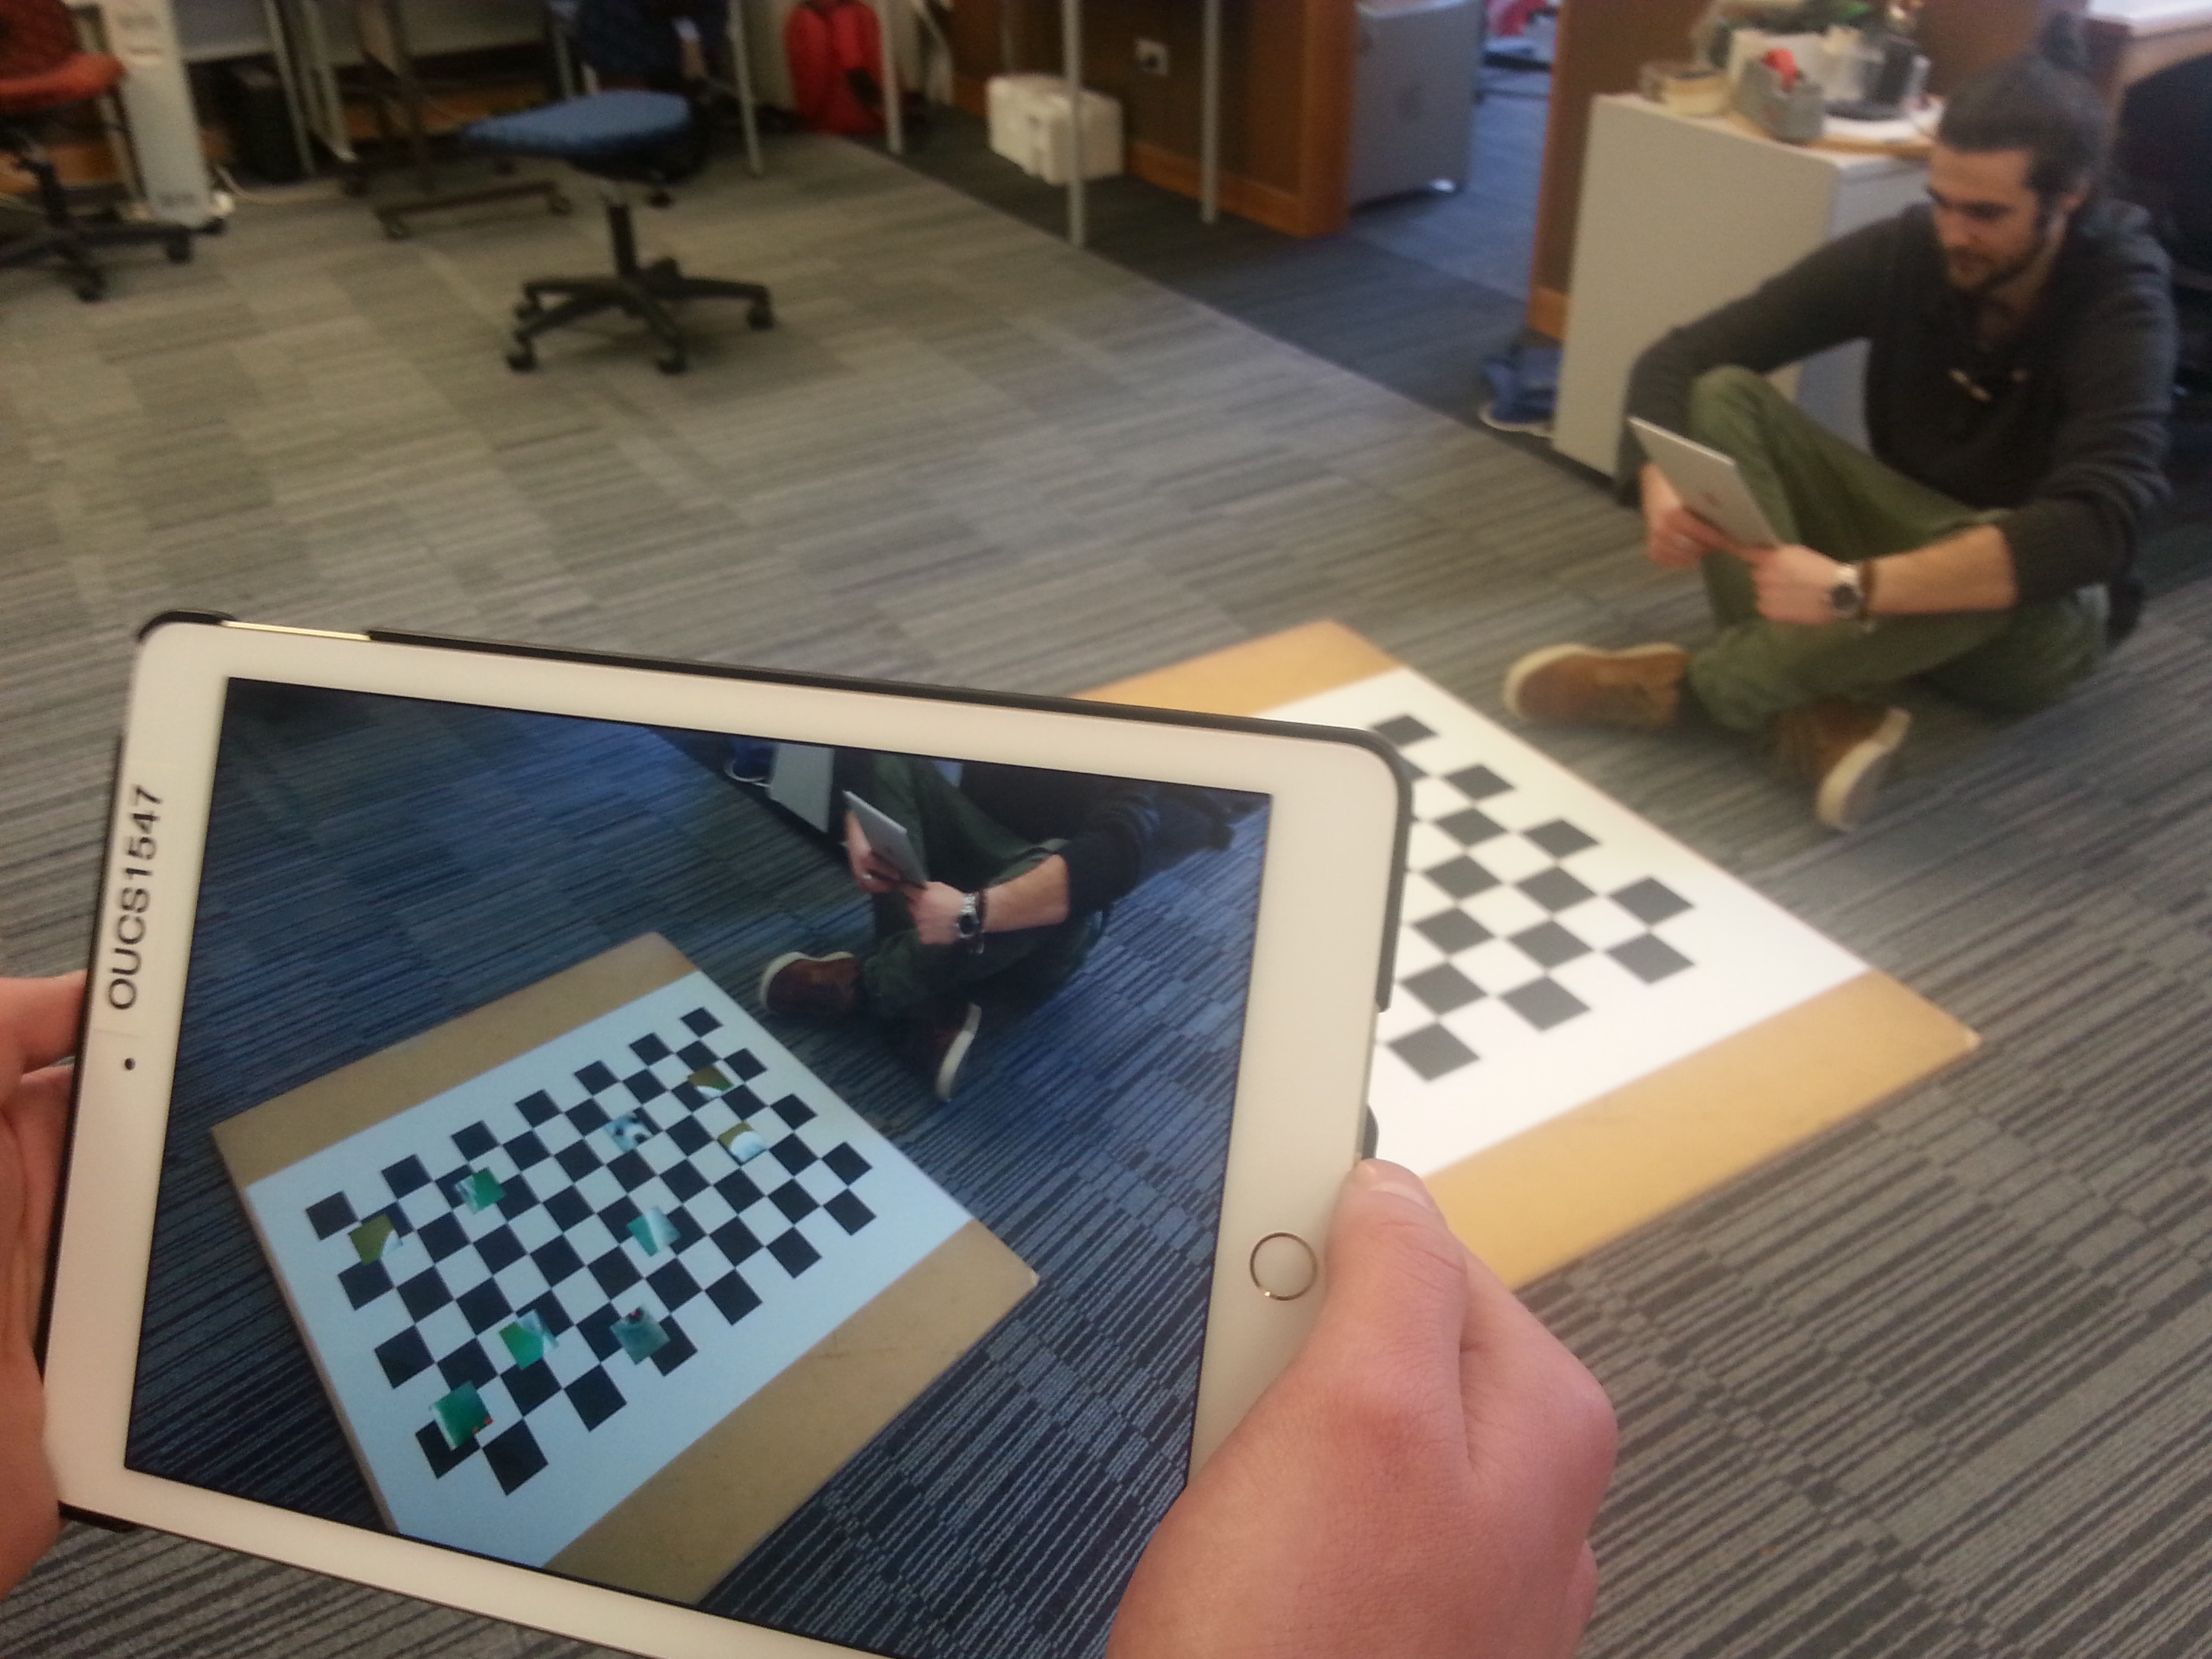
\includegraphics[width=1\textwidth]{images/BigBoardImage}
\caption{Screenshot of us playing on a large game board.}
\label{fig:BigGameBoard}
\end{center}
\end{figure}

% What hasn't been done
\subsection{Future Work}
There were still several things that I have missed out on implementing for the
game logic and rendering of the Giguesaur application. Firstly, puzzle pieces
are still only simple square polygons. For future recommendations, this would be
changed so that pieces have curved edges, similar to Figure
\ref{fig:FarmsAnimals} earlier in the document. The curved edges to pieces would
make the virtual jigsaw puzzle look more like a conventional jigsaw puzzle, and
it would allow for players to easily solve the puzzle rather than having to
match the images on the current puzzle pieces. This could be implemented using a
random number generator that would choose a certain number of points along each
piece's edge, and than map vertices along each point, which would hopefully
generate a curve.\\

Secondly, the application is quite slow, with it only running at a maximum of
five frames per second. This is caused by the OpenCV functions that compute the
perspective projection matrix. The routines are looking for a checkerboard
pattern every frame from the camera. Another slow down to the application could
be due to how we are rendering the game, as each frame from the camera is being
processed and sent to the OpenGL code for rendering. If we had more time to
experiment we could attempt to try have the puzzle pieces being rendered on top
of the video feed coming from the camera.\\

Finally, there is no real way to know when you as a player are holding a puzzle
piece. As of right now, when a player picks up a puzzle piece it moves to the
centre of the screen and than gets projected onto the game board. This would be
used to show where, if the player were to tap the screen, the piece would be
placed back onto the board. What should be happening is when a player picks up a
piece it should show a larger image of the puzzle piece in the centre of the
screen with it being partially transparent, and be casting a shadow where the
piece will appear on the game board.

\subsection{Final Thoughts}
The Giguesaur project has been a challenging and fun experience for me. I have
learnt a lot about developing a large piece of software while collaborating with
a team. I would have loved to have had more time to do further work on the
project to implement the future work, but alas, time was not on our side.

%---------------------------------------------------------------------------
% References
%---------------------------------------------------------------------------

\clearpage

\bibliographystyle{ieeetr}
\bibliography{references}

%---------------------------------------------------------------------------
% Glossary
%---------------------------------------------------------------------------

\clearpage
\printglossaries

%---------------------------------------------------------------------------
% End
%---------------------------------------------------------------------------

\end{document}
